\subsection{Περιβάλλον υλοποίησης}

\subsubsection{Unity Editor}

\textbf{Εγκατάσταση}

Η εγκατάσταση του Unity Editor γίνεται μέσω του Unity Hub, το οποίο είναι μια αυτόνομη εφαρμογή με σκοπό την πρόσβαση στο οικοσύστημα Unity. Το Hub προσφέρει εύκολη διαχείριση των Unity projects και των αδειών για τα Unity λογισμικά, καθώς και προσφέρει τη δυνατότητα εγκατάστασης πρόσθετων στοιχείων (add-ons) και πολλών εκδόσεων του Unity Editor.

\begin{figure}[H]
    \centering
    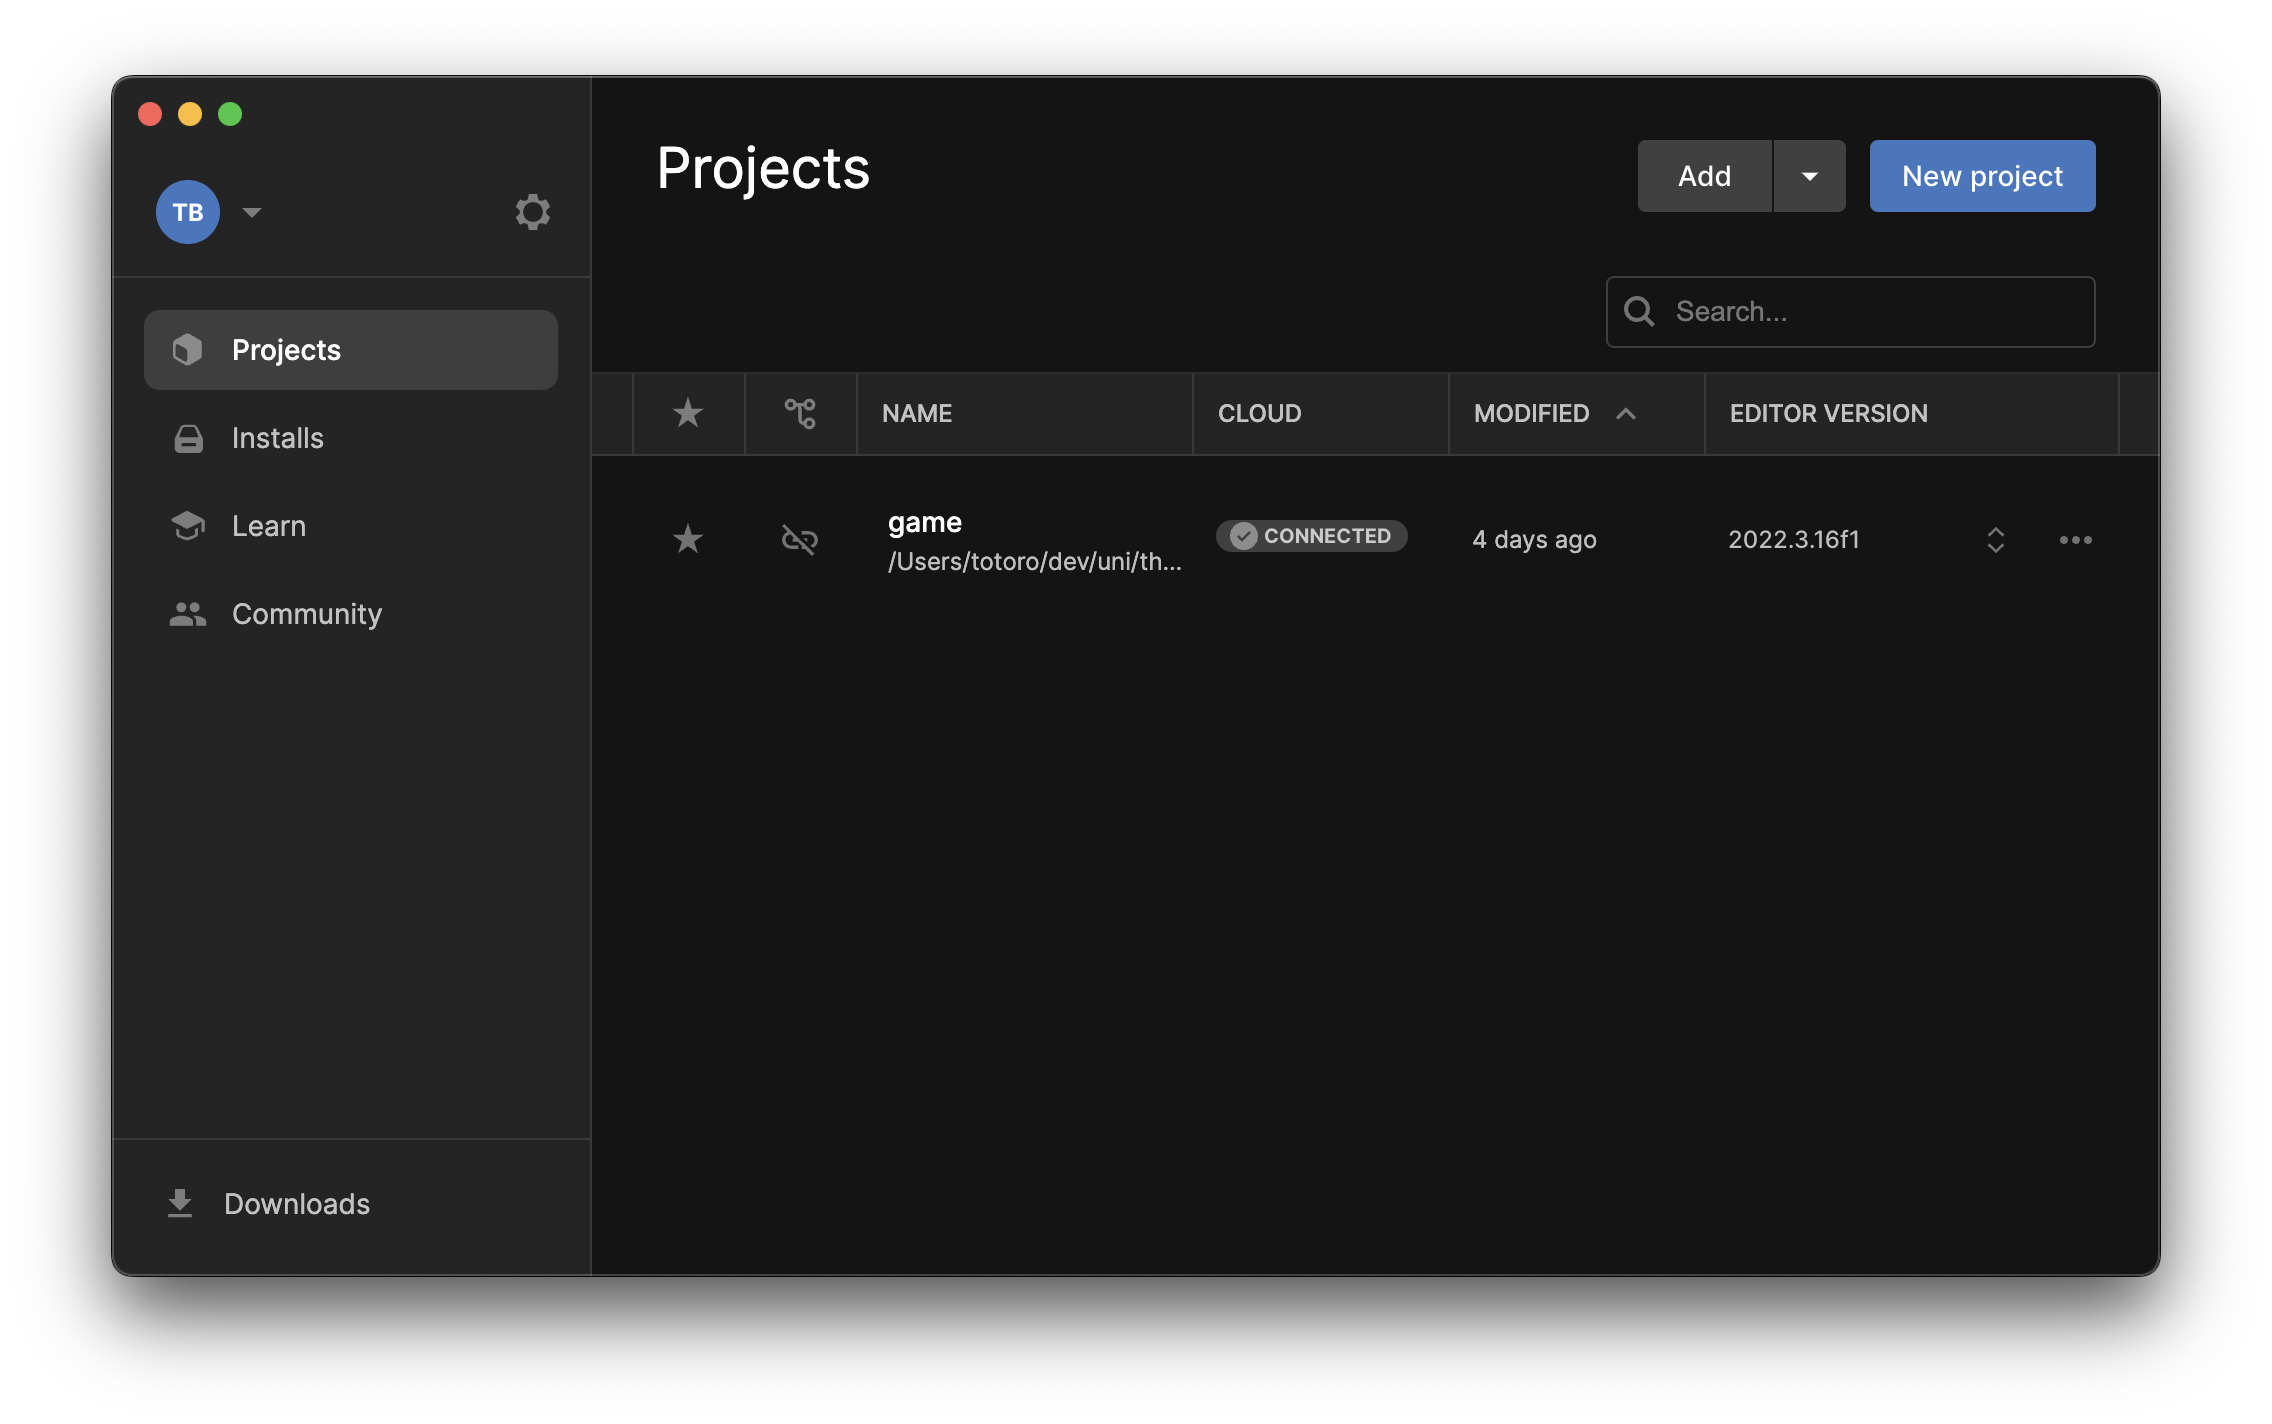
\includegraphics[width=1\linewidth]{sections/4/1/images/unity_hub}
    \caption{Το Unity Hub}
    \label{fig:unity_hub}
\end{figure}

Για τη δημιουργία του παιχνιδιού επιλέχθηκε το Unity Editor 2022.3.16f1 διότι ήταν η τελευταία τότε έκδοση \acrshort{lts}.

% ========================================

\pagebreak
\showheader

\textbf{Πρώτη ματιά}

Το Unity Editor προσφέρει μία φιλική προς το χρήστη διεπαφή η οποία αποτελείται από πολλά παράθυρα με διάφορους σκοπούς τα οποία μπορούν να τοποθετηθούν και να αποσυνδεθούν κατά βούληση. Αυτό προσφέρει τη δυνατότητα στο κάθε χρήστη να τα τοποθετήσει όπως εκείνος επιθυμεί.

\begin{figure}[H]
    \centering
    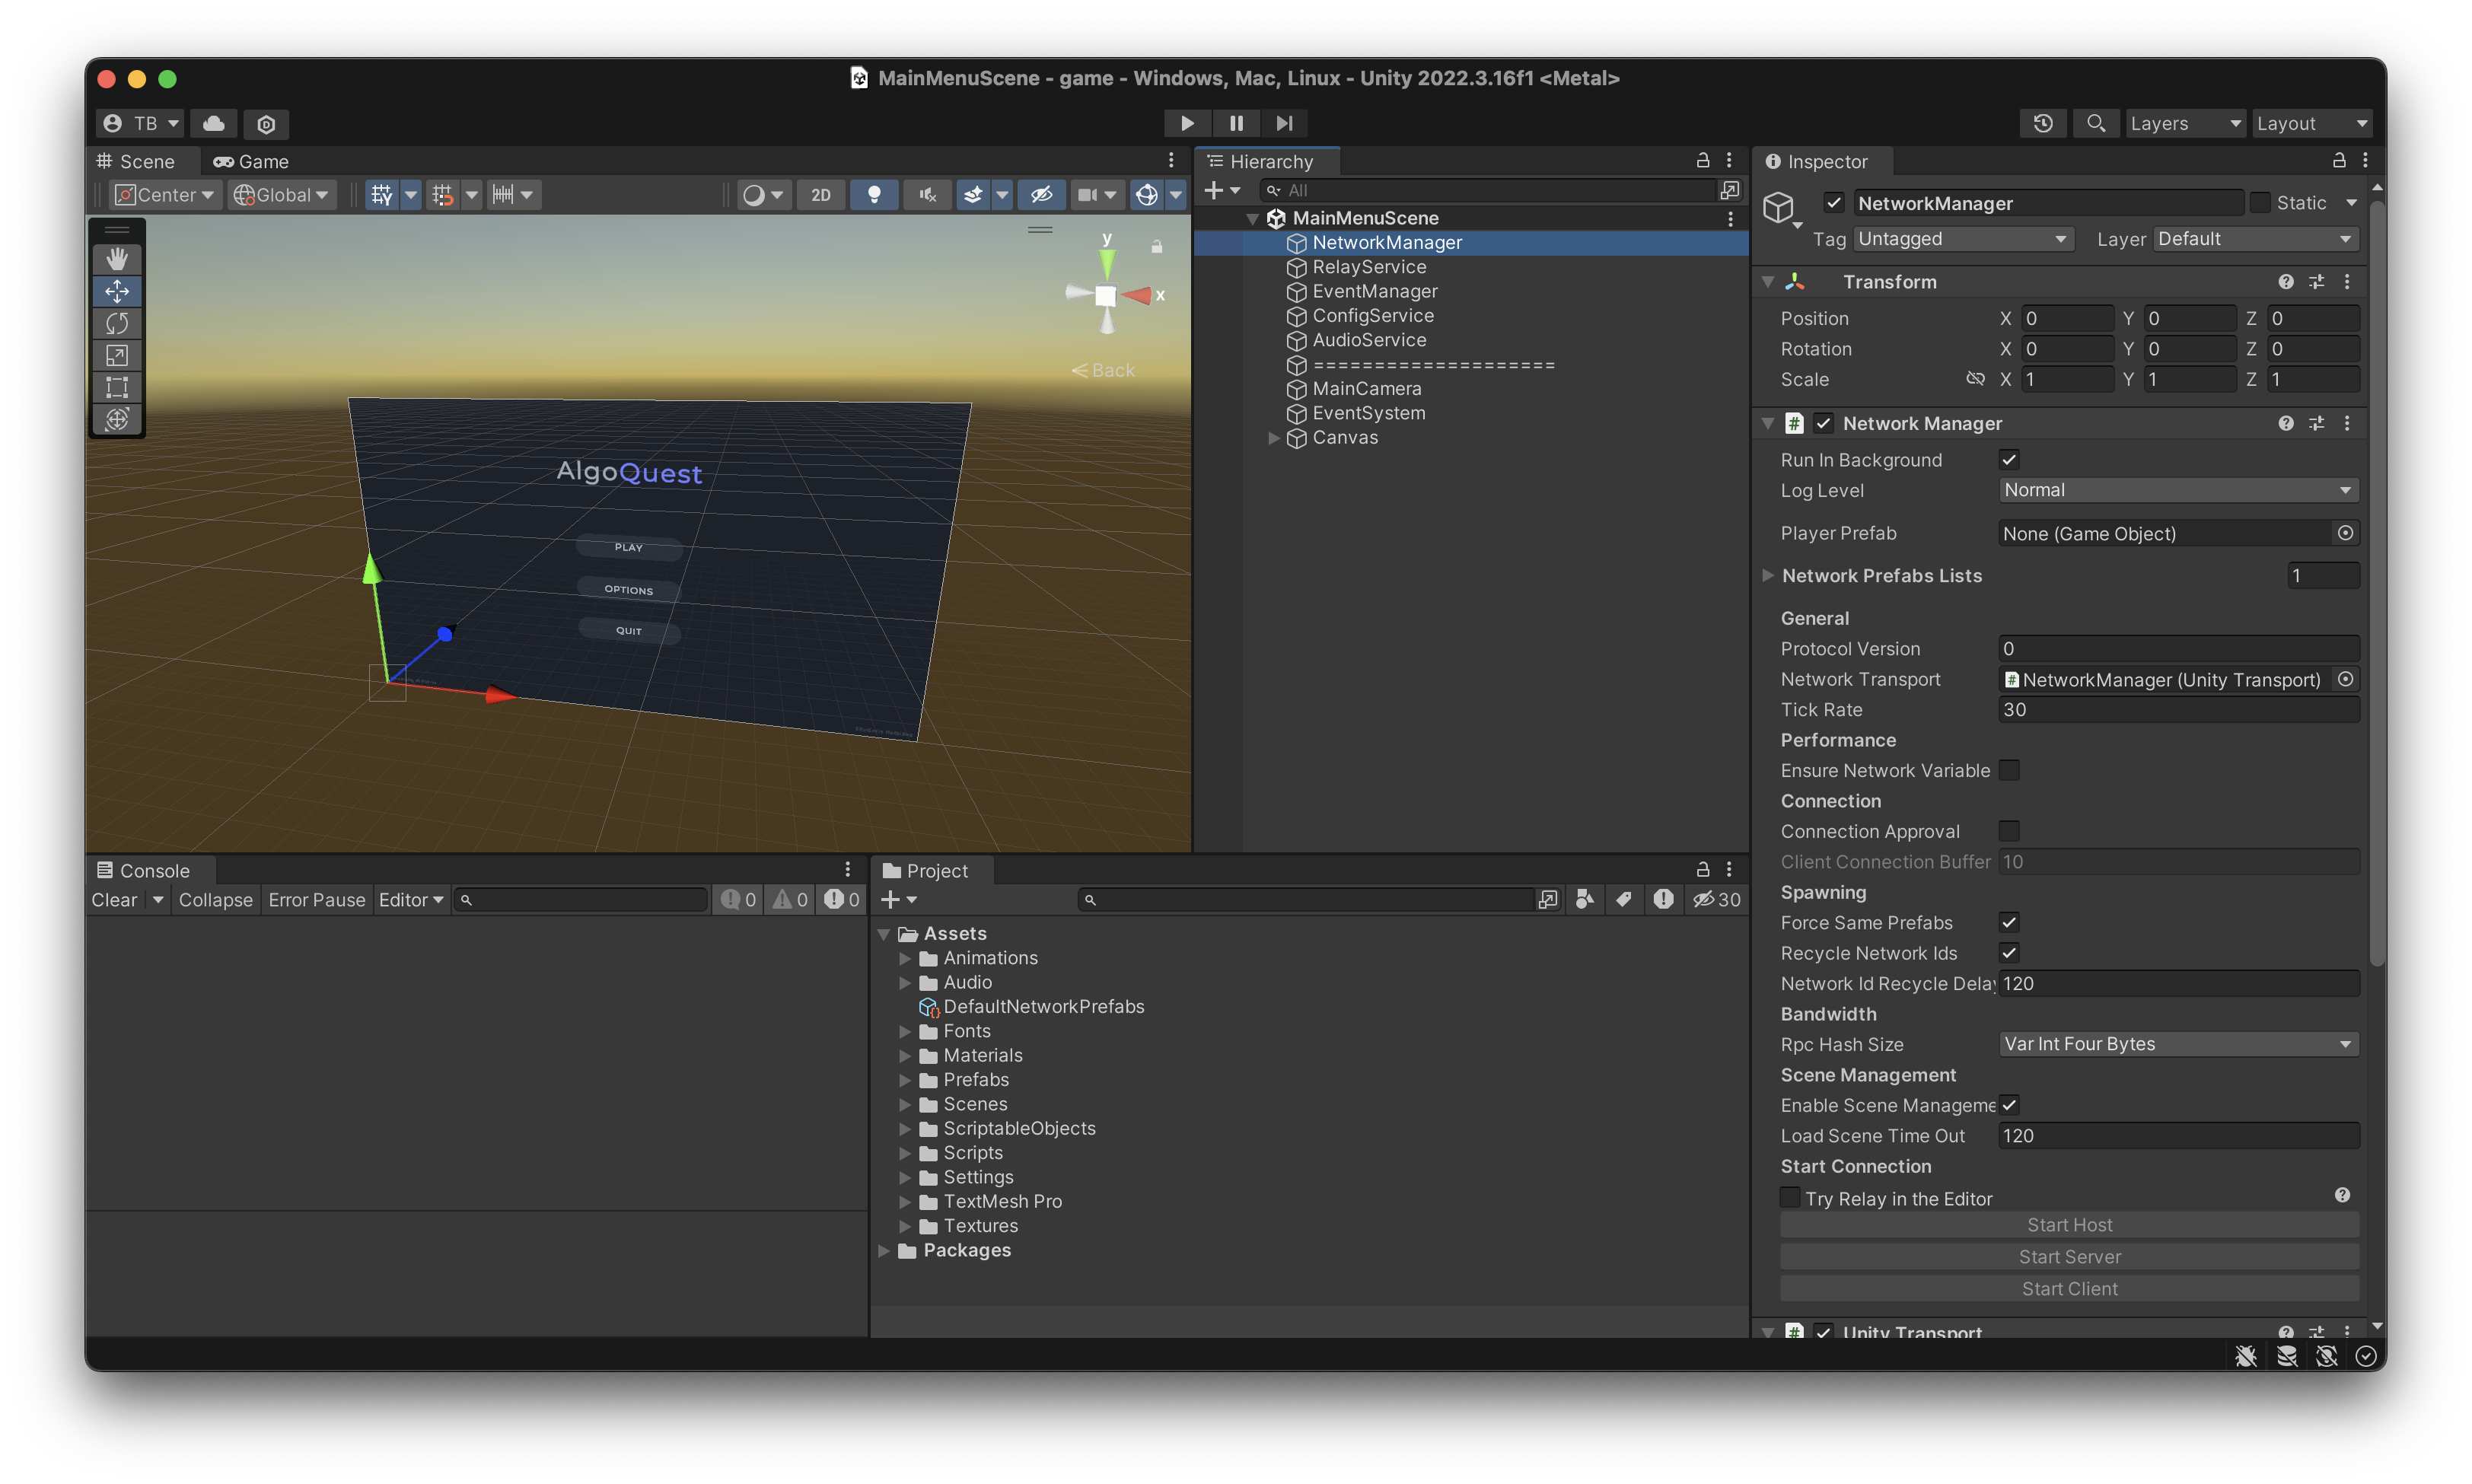
\includegraphics[width=1\linewidth]{sections/4/1/images/unity_editor}
    \caption{Το Unity Editor}
    \label{fig:unity_editor}
\end{figure}

Τα παράθυρα που προσφέρει το Unity Editor είναι αρκετά για να καλύψουν κάθε ανάγκη που μπορεί να έχει κάποιος ο οποίος θέλει να κατασκευάσει ένα παιχνίδι χρησιμοποιώντας την εφαρμογή. Από αυτά τα βασικότερα που χρησιμοποιήθηκαν κατά την κατασκευή αυτού του παιχνιδιού είναι τα εξής:

\begin{itemize}
    \item \textbf{Hierarchy (Εικόνα \ref{fig:unity_editor} πάνω-κέντρο):} Το παράθυρο αυτό περιέχει μία ιεραρχική μορφή όλων των GameObjects που υπάρχουν στην επιλεγμένη σκηνή. Ο χρήστης μπορεί να μετακινήσει κάποιο GameObject σε οποιοδήποτε μέρος του δέντρου επιθυμεί.
    \item \textbf{Scene (Εικόνα \ref{fig:unity_editor} πάνω-αριστερά):} Αυτό είναι το παράθυρο τρισδιάστατης προβολής του κόσμου το οποίο μπορεί να χρησιμοποιήσει ο χρήστης για να μετακινηθεί, καθώς και να ελέγξει τον κόσμο και τα GameObjects που βρίσκονται μέσα σε αυτόν.
    \item \textbf{Inspector (Εικόνα \ref{fig:unity_editor} δεξιά):} Αναμφισβήτητα το πιο σημαντικό παράθυρο του Unity Editor, το Inspector εμφανίζει όλα τα Components του επιλεγμένου GameObject. Με τη χρήση αυτών των components ο χρήστης μπορεί να διαχειριστεί την θέση του GameObject στον κόσμο, αλλά και την συμπεριφορά του σε αυτόν.
    \item \textbf{Console (Εικόνα \ref{fig:unity_editor} κάτω-αριστερά):} Σε αυτό το παράθυρο εμφανίζονται όλα τα logs της εφαρμογής κατά τη διάρκεια της κατασκευής, τα οποία μπορεί να είναι είτε λάθη που μπορεί να συμβούν στο παιχνίδι, είτε logs που ο ίδιος ο χρήστης έχει τοποθετήσει στον κώδικα του.
    \item \textbf{Project (Εικόνα \ref{fig:unity_editor} κάτω-κέντρο):} Εδώ εμφανίζονται όλα τα αρχεία που υπάρχουν στους φακέλους του project, είτε του ίδιου του χρήστη (φάκελος Assets) είτε του Unity και των πρόσθετων πακέτων που μπορεί να έχει κατεβάσει ο χρήστης (φάκελος Packages).
\end{itemize}

Σε αυτό το σημείο είναι σημαντικό να σημειωθεί πως το Unity Editor και τα παράθυρα του είναι μία συλλογή από scripts. Αυτό σημαίνει, πως εκτός από τη συνηθισμένη χρήση των scripts που γράφει ένας χρήστης, τα οποία αφορούν την συμπεριφορά των GameObjects στον κόσμο, μπορεί κάποιος να γράψει scripts τα οποία δημιουργούν παράθυρα για κάποιο ειδικό σκοπό. Οι πιθανές χρήσεις τους μπορεί να είναι σχετικά απλές, όπως η δημιουργία παραθύρου για \glspl{cheat_code} ή αρκετά περίπλοκες, όπως για τον έλεγχο της συμπεριφοράς GameObject σε κάποιο cutscene όπως βλέπουμε στην εικόνα \ref{fig:unity_custom_editor_windows}\cite{technologies_unity_nodate}.

\begin{figure}[H]
    \centering
    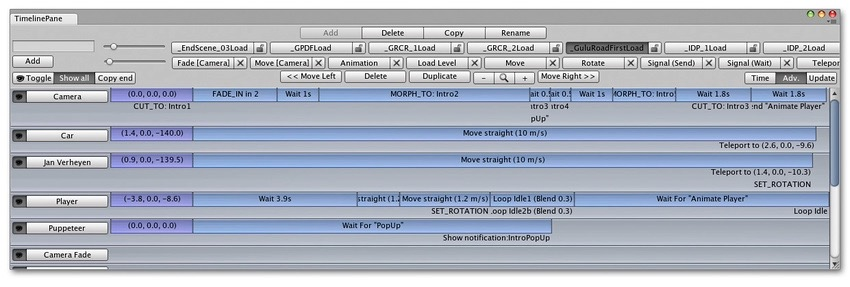
\includegraphics[width=1\linewidth]{sections/4/1/images/unity_custom_editor_windows}
    \caption{Unity παράθυρο ειδικού σκοπού που χρησιμοποιείται για τον έλεγχο της συμπεριφοράς GameObject σε cutscene}
    \label{fig:unity_custom_editor_windows}
\end{figure}

\textbf{Scenes}

Η κατασκευή εφαρμογών στο Unity γίνεται με τη χρήση σκηνών (Scenes), όπου κάθε σκηνή είναι ένα ξεχωριστό επίπεδο ή περιβάλλον μέσα στο project. Σε αυτές τοποθετούνται διάφορα GameObjects όπως χαρακτήρες, φωτισμός και κάμερες τα οποία μπορούν να ρυθμιστούν και να αλληλεπιδρούν μέσα σε αυτές τις σκηνές.

Χρησιμεύουν επίσης ως δοχεία από GameObjects τα οποία κάνουν εύκολη την οργάνωση και σχεδίαση του κόσμου μιας εφαρμογής, καθώς μοιράζουν τον εικονικό κόσμο σε εύκολα διαχειρίσιμα τμήματα.

Λόγω της αρθρωτής φύσης τους, οι σκηνές διευκολύνουν τις ομαλές μεταβάσεις μεταξύ διαφορετικών τμημάτων μιας εφαρμογής, όπως η πλοήγηση από ένα μενού σε ένα περιβάλλον παιχνιδιού.

\textbf{GameObjects}

Το θεμελιώδες δομικό στοιχείο μιας εφαρμογής στο Unity, το GameObject, αντιπροσωπεύει μία οντότητα σε μία σκηνή. Κάθε στοιχείο σε μία σκηνή, είτε πρόκειται για χαρακτήρα, είτε για σκηνικό, είτε για περιβαλλοντικό χαρακτηριστικό, είναι μία περίπτωση ενός GameObject. Με διάφορους συνδυασμούς Components μπορούν να μετατραπούν σε οτιδήποτε, από ένα φόντο σε ένα μενού μέχρι έναν πολύπλοκο και διαδραστικό χαρακτήρα παίκτη.

Το Unity προσφέρει μια εναλλακτική λύση για υλοποίηση εφαρμογής αντί για GameObjects, το \acrfull{unity_ecs}\cite{noauthor_entity_nodate}, μέρος του \acrfull{unity_dots} του Unity\cite{noauthor_dots_nodate}, το οποίο έχει μεγαλύτερο προσανατολισμό στην απόδοση. Τα Entities είναι ελαφριά δοχεία δεδομένων τα οποία διαχωρίζουν τα δεδομένα και τη συμπεριφορά ενός αντικειμένου, με σκοπό τη μεγιστοποίηση της αποδοτικότητας του χρόνου εκτέλεσης και την καλύτερη χρήση των επεξεργαστών με πολλαπλούς πυρήνες. Η χρήση τους, δυστυχώς, δεν είναι τόσο διαδεδομένη όσο των GameObjects με αποτέλεσμα να υπάρχουν λιγότεροι πόροι βοήθειας, καθώς και χαμηλότερη υποστήριξη από την κοινότητα του Unity. Αυτός είναι και ο λόγος για τον οποίο επιλέχθηκαν τα GameObjects για αυτή την εφαρμογή.

\textbf{Components}

Τα Components είναι βασικά στοιχεία τα οποία τοποθετούνται σε GameObjects και καθορίζουν τη συμπεριφορά, την εμφάνιση και τη λειτουργικότητα τους. Είναι αυτά που δίνουν στα GameObjects τις ξεχωριστές τους ιδιότητες και δυνατότητες μέσα σε ένα Scene.

Υπάρχουν διάφοροι τύποι Components που μπορούν να χρησιμοποιηθούν στα GameObjects, όπως:

\begin{itemize}
    \item \textbf{Transform Components:} Κάθε GameObject περιλαμβάνει εξ ορισμού ένα Component Transform, το οποίο καθορίζει τη θέση, την περιστροφή και την κλίμακα του GameObject στο Scene.
    \item \textbf{Physical Components:} Περιλαμβάνουν Rigidbody και Colliders που επιτρέπουν αλληλεπιδράσεις βασισμένες στη φύση, όπως η βαρύτητα και οι συγκρούσεις.
    \item \textbf{Visual Components:} Μπορεί να είναι Mesh Renderer Components, τα οποία είναι υπεύθυνα για την εμφάνιση των μοντέλων των GameObjects, ή ακόμη και Light Components τα οποία επηρεάζουν τον φωτισμό και τις σκιές.
    \item \textbf{Audio Components:} Audio Source ή Audio Listener Components τα οποία χρησιμοποιούνται για την αναπαραγωγή ήχων και τη διαχείριση του τρόπου με τον οποίο ο ήχος γίνεται αντιληπτός στο περιβάλλον.
    \item \textbf{Scripts:} Κώδικες γραμμένοι συνήθως σε C\#\cite{noauthor_c_nodate}, μπορούν να προστεθούν ως Components για τον έλεγχο της συμπεριφοράς των GameObject μέσω κώδικα.
\end{itemize}

\textbf{Scripts}

Τα Script μπορούν να χρησιμοποιηθούν για τον έλεγχο της εφαρμογής μέσω κώδικα. Συνήθως γραμμένα σε C\#, μπορούν είτε να προστεθούν σε Components εφόσον κληρονομούν από την κλάση \verb|MonoBehaviour| που παρέχει το Scripting API του Unity (ή την \verb|NetworkBehaviour| εφόσον χρειάζεται λειτουργικότητα στο δίκτυο), είτε σαν δεδομένα που μπορούν να μοιράζονται μεταξύ πολλών Script, εφόσον κληρονομούν από την κλάση \verb|ScriptableObject|, είτε να χρησιμοποιηθούν σαν απλά Scripts που προσφέρουν παραπάνω λειτουργικότητα σε άλλα Script, όπως το να επικοινωνούν με εξωτερικές υπηρεσίες.

Τα Scripts που κληρονομούν από την κλάση \verb|MonoBehaviour| προσφέρουν τη δυνατότητα να επικοινωνούν με το Unity Editor και να διαχειρίζονται τη συμπεριφορά των GameObjects.
\begin{itemize}
    \item \textbf{Event functions:} Συναρτήσεις συμβάντων που συμβαίνουν σε διαφορετικά στάδια της ζωής μιας εφαρμογής. Μερικές από αυτές είναι:
    \begin{itemize}
        \item \verb|OnEnable()| και \verb|OnDisable()|: Καλούνται όταν το GameObject ενεργοποιείται ή απενεργοποιείται αντίστοιχα.
        \item \verb|Awake()|: Καλείται όταν το GameObject δημιουργείται.
        \item \verb|Start()|: Καλείται πριν το πρώτο καρέ της εφαρμογής.
        \item \verb|Update()|: Καλείται κάθε καρέ της εφαρμογής.
    \end{itemize}
    \item \textbf{Coroutines:} Είναι μέθοδοι οι οποίες μπορούν να διακόψουν την εκτέλεση του Script και να επιστρέψουν τον έλεγχο στο Unity, αλλά στη συνέχεια να συνεχίσουν από εκεί που σταμάτησαν σε επόμενα καρέ.
    \item \textbf{Physics events:} Μέθοδοι συμβάντων οι οποίες μπορούν να χρησιμοποιηθούν για το χειρισμό της φυσικής και των συγκρούσεων. Οι βασικότερες από αυτές, \verb|OnCollisionEnter()| και \verb|OnTriggerEnter()|, ανταποκρίνονται στις αλληλεπιδράσεις της φυσικής αν το GameObject έχει κάποιο Collider Component.
    \item \textbf{Messaging system:} Η κλάση \verb|MonoBehaviour| περιλαμβάνει ένα σύστημα μυνημάτων, το οποίο επιτρέπει σε Scripts να στέλνουν και να λαμβάνουν μηνύματα που μπορούν να καλέσουν μεθόδους. Συναρτήσεις όπως \verb|SendMessage()| και \verb|BroadcastMessage()| επιτρέπουν αυτή την επικοινωνία μεταξύ Scripts.
    \item \textbf{Lifecycle control:} Περιλαμβάνει μεθόδους που μπορούν να χρησιμοποιηθούν για τον έλεγχο της ζωής του GameObject, όπως \verb|Destroy()| η οποία καταστρέφει ένα GameObject από ένα Scene ή \verb|OnDestroy()| που καλείται όταν το GameObject καταστρέφεται.
    \item \textbf{Editor control:} Scripts που κληρονομούν από την κλάση \verb|MonoBehaviour| μπορούν να εμφανίσουν πεδία στο Unity Editor τα οποία αντιστοιχούν σε μεταβλητές μέσα στα αντίστοιχα Script. Αυτό επιτρέπει τον έλεγχο και τη ρύθμιση παραμέτρων του GameObject χωρίς να χρειάζεται να χτιστεί κάθε φορά το Script, καθώς και εύκολο έλεγχο του GameObject από άτομα τα οποία δεν έχουν γνώσεις σε γλώσσες προγραμματισμού.
\end{itemize}

\begin{figure}[H]
    \centering
    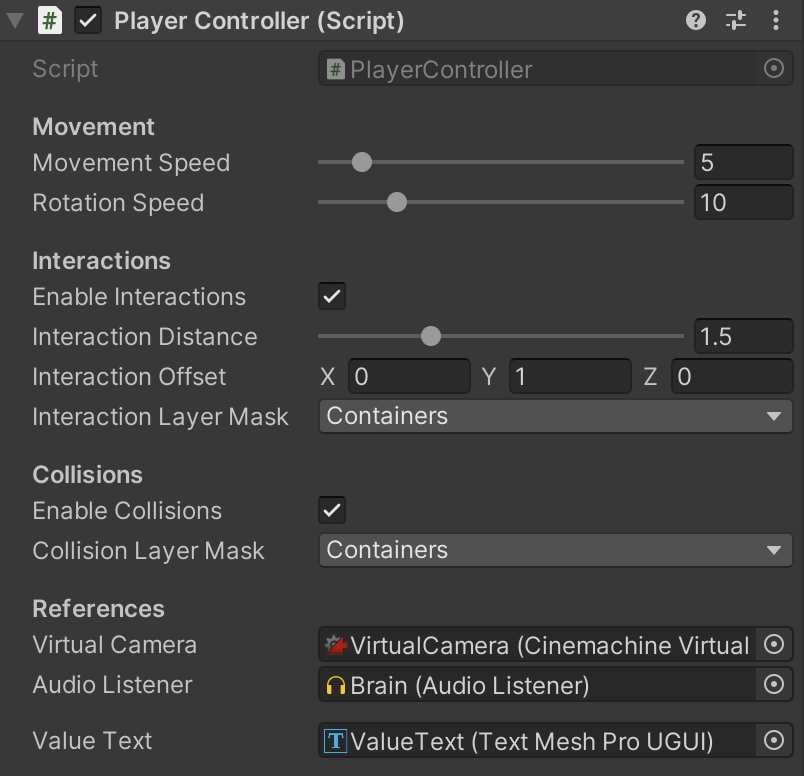
\includegraphics[width=0.6\linewidth]{sections/4/1/images/unity_editor_player_controller}
    \caption{Script ελέγχου του παίκτη με πεδία στο Unity Editor}
    \label{fig:unity_editor_player_controller}
\end{figure}

Τα Scripts που κληρονομούν από την κλάση \verb|ScriptableObject| επιτρέπουν στους χρήστες να δημιουργούν αντικείμενα τα οποία δεν χρειάζεται να είναι συνδεδεμένα με κάποιο GameObject. Παρέχουν ένα τρόπο αποθήκευσης δεδομένων ανεξάρτητο από Scenes ή GameObjects, προσφέροντας έτσι έναν εύκολο τρόπο διαχείρισης κοινών δεδομένων σε μία εφαρμογή.

Ένα ακόμη καλό των \verb|ScriptableObject| είναι πως δημιουργούνται μέσω του \gls{context_menu} προσφέροντας έτσι έναν εύκολο τρόπο σε χρήστες που δεν έχουν γνώσεις στον προγραμματισμό να διαχειριστούν την εφαρμογή.

Συγχρόνως προσφέρουν οργάνωση και αποδοτικότητα καθώς αποθηκεύονται σε ένα σημείο και όχι σε κάθε GameObject οπότε μειώνουν τον χώρο αποθήκευσης που χρειάζεται κάποιος για την εφαρμογή, καθώς και προσφέρουν ένα κεντρικό σημείο από το οποίο μπορεί κάποιος να ρυθμίσει μεταβλητές της εφαρμογής. Αυτό μπορεί να συμβεί και κατά τη διάρκεια του παιχνιδιού στο Unity Editor, κάτι το οποίο δεν ισχύει για τις ρυθμίσεις πάνω σε ένα GameObject.

\begin{figure}[H]
    \centering
    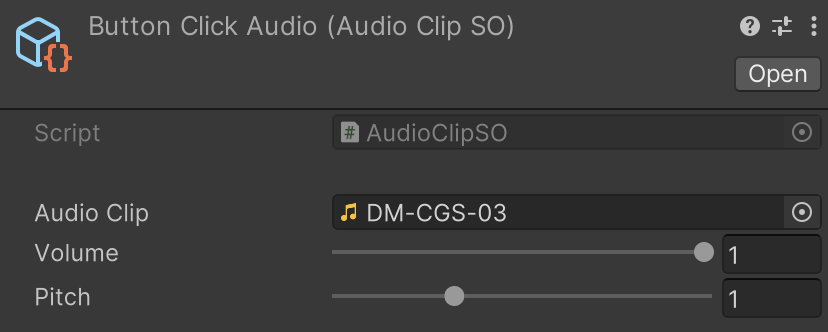
\includegraphics[width=0.6\linewidth]{sections/4/1/images/unity_editor_button_click_audio_so}
    \caption{ScriptableObject για τον έλεγχο του ήχου που παίζει όταν κάποιος παίκτης κάνει κλικ σε ένα κουμπί}
    \label{fig:unity_editor_button_click_audio_so}
\end{figure}
